\section{Theorie}
\label{sec:Theorie}

\subsection{Einleitung}

Innerhalb dieses Experiments wird die Funktionsweise eines Helium-Neon Lasers untersucht.


\subsection{Funktionsweise eines Lasers}

Die wesentliche Eigenschaft eines Lasers ist, dass er mit Hilfe von stimulierter
Emission in der Lage ist, monochromatisches Licht mit hoher Intensität und
hoher Kohärenz zu erzeugen.
Um einen Laser zu realisieren werden im Allgemeinen drei Komponenten benötigt:
eine Pumpquelle, ein Lasermedium und ein Resonator. Im Lasermedium muss durch die zugeführte
Energie der Pumpquelle eine Besetzungsinversion induziert werden können
damit der Laser überhaupt funktionieren kann. Um dies genauer zu verstehen,
werden im folgenden Abschitt zunächst verschiedene Arten von Emission und Absorption
anhand eines Zweiniveausystems erklärt.

Im thermodynamischen Gleichgewicht und ohne äußere Energiezufuhr ist der Grundzustand im
Zweiniveausystem stärker besetzt als der angeregte Zustand. Pumpt man Photonen mit einer Energie,
die der Energiedifferenz der beiden Niveaus entspricht, in das System, so werden diese mit der Rate
\begin{align}
  \frac{\mathrm{d}{N}_A}{\mathrm{d}t} = n_1 \rho(\nu) B_{12}
\end{align}
absorbiert, wobei ein Elektron vom Grundzustand in den angeregten Zustand angehoben wird. Dabei ist $n_1$
die Besetzungszahl des Grundzustands, $\rho(\nu)$ das Strahlungsfeld und $B_{12}$ ein sogenannter
Einsteinkoeffizient. Andersherum kann ein Elektron auch unter Emission eines Photons vom angeregten
Zustand in den Grundzustand übergehen. Dabei wird zwischen spontaner Emission, die unabhängig vom
externen Strahlungsfeld auftritt gemäß der Rate
\begin{align}
  \frac{\mathrm{d}{N}_\text{spont}}{\mathrm{d}t} = n_2 A_{21},
\end{align}
und induzierter Emission, deren Rate
\begin{align}
  \frac{\mathrm{d}{N}_\text{ind}}{\mathrm{d}t} = n_2 \rho(\nu) B_{21}
\end{align}
proportional zum Strahlungsfeld ist, unterschieden. Bei der spontanen Emission werden Photonen in beliebige
Richtung und beliebiger Phase emittiert, während bei der induzierten Emission Phase und Richtung von einfallendem
Photon und ausfallenden Photonen übereinstimmen. Alle drei beschriebenen Fälle sind in Abbildung
\ref{fig:absemi} skizziert. Sind die Zustände des Zweiniveausystems nicht entartet, so gilt für die
Einsteinkoeffizienten
\begin{align}
  B_{12} = B_{21} = B.
\end{align}
Es folgt sofort, dass in diesem System keine Besetzungsinversion erzeugt werden kann, denn die
gesamte Rate für Übergänge vom angeregten Zustand in den Grundzustand ist in jedem Fall bei
einer Besetzung von $n_1 = n_2 = 0.5$ größer, als die Rate für Übergänge in die andere Richtung.
Entsprechend ist ein Zweiniveausystem ungeeignet als Lasermedium.

\begin{figure}[H]
  \centering
  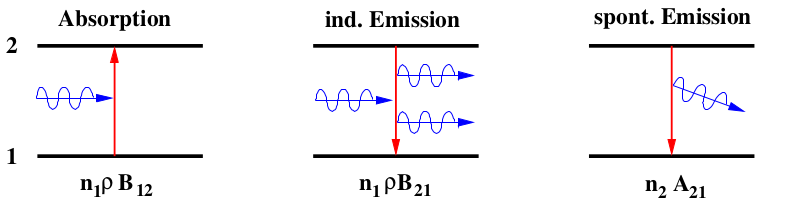
\includegraphics[height = 3.7cm]{Pics von Buddy/absemi.png}
  \caption{Strahlungsübergänge in einem Zweiniveausystem \cite{anleitung}.}
  \label{fig:absemi}
\end{figure}

Der Grund, warum eine Besetzungsinversion für das Lasen erforderlich ist, liegt darin, dass das
Strahlungsfeld sich nur dann beim Durchgang durch das Medium selbst verstärken kann.
Ein Dreiniveausystem beispielsweise, wie es in Abbildung \ref{fig:dreiniveau} zu sehen ist,
erfüllt diese Bedingung unter bestimmten Voraussetzung.
Dafür werden Elektronen vom Grundzustand in den höchst angeregten dritten Zustand gepumpt.
Eine wichtige Notwendigkeit ist, dass der anschließende Übergang vom höchsten in
den mittleren Zustand schnell geschieht, der dritte Zustand also instabil ist. Damit werden
die Elektronen letzlich indirekt vom Grundzustand in den ersten angeregten Zustand gepumpt.
Das indirekte Pumpen hat den Vorteil, dass keine Strahlungsübergänge via induzierte Emission
durch die Pump Photonen vom mittleren Niveau in den Grundzustand mehr auftreten, da die
Energiedifferenz eine andere ist. Dadurch kann erreicht werden, dass die Rate, mit welcher
das zweite Niveau befüllt wird, auch bei einer Besetzung von $n_1 = n_2 = 0.5$ noch größer,
als die Rate mit welcher der Grundzustand befüllt wird, ist und eine Besetzungsinversion
erzeugt werden. Fällt bei diesen Gegebenheiten nun ein Strahlungsfeld $\rho$ mit
der entsprechenden Photonenergie ein, so induziert dieses wegen der Besetzungsinversion mehr
Emissionen als Absorptionen, sodass es sich selbst durch das Lasermedium verstärkt.
Diese Verstärkung der Lichtintensität verläuft exponentiell mit der Strecke, die der Lichtstrahl
durch das aktive Lasermedium zurücklegt. Durch den oben bereits aufgezählten Resonator kann diese
Strecke erheblich vergrößert werden, sodass ein intensiver Laserstrahl erzeugt wird.
Wie genau das funktioniert wird im folgenden Abschnitt erläutert.

\begin{figure}[H]
  \centering
  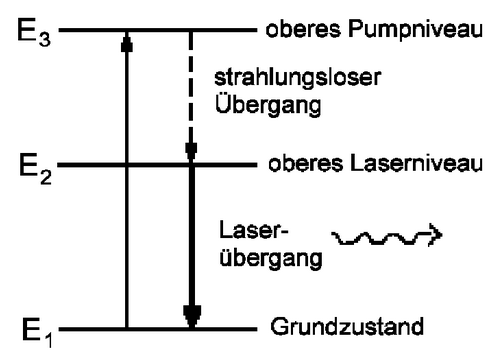
\includegraphics[height = 4.4cm]{Pics von Buddy/dreiniveau.png}
  \caption{Strahlungsübergänge in einem Dreiniveausystem \cite{laser}.} %http://www.pci.tu-bs.de/aggericke/PC4/Kap_III/Laser.htm
  \label{fig:dreiniveau}
\end{figure}

Der grundlegende Aufbau eines Lasers ist in Abbildung \ref{fig:laseraufbau} erkennbar.
Zwei Spiegel, die um das Lasermedium platziert werden, reflektieren den austretenden
Lichtstrahl zurück in das Medium, wo er sich selbst verstärkt. Einer der Spiegel ist
teildurchlässig mit einem Transmissionskoeffizienten von etwa $1-2 \, \si{\percent}$,
damit der erzeugte Laserstrahl ausgekoppelt werden kann. 

\begin{figure}
  \centering
  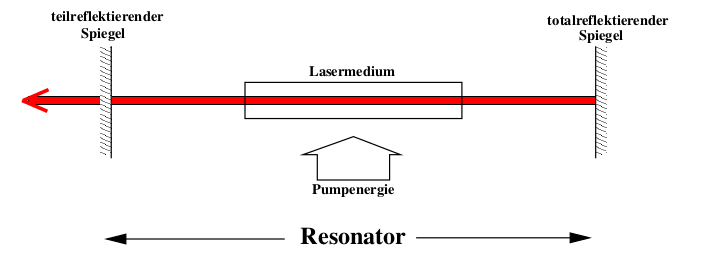
\includegraphics[height=5cm]{Pics von Buddy/laseraufbau.png}
  \caption{\cite{anleitung}.}
  \label{fig:laseraufbau}
\end{figure}
